\begin{tframe}{Validation}

The faces used in the training of the models might not be completely clean.

\vspace{0.1in}

For example, if an image contains two faces, each of them will have the same ranking; thus, if the ranking is high, they will both be used in the training phase but only one of them will correctly represent the identity. 

\vspace{0.1in}

Since it is not possible to resolve these problems in the previous steps, we have classification models that have been obtained with a training set containing errors.

\end{tframe}


\begin{tframe}{Validation}

\begin{figure}[h]
\begin{center}
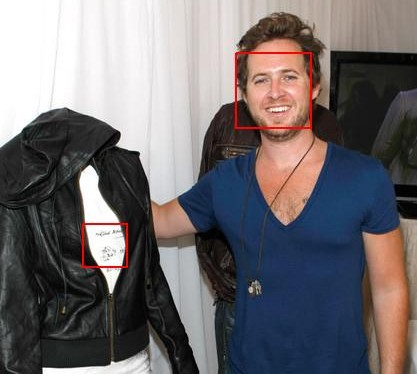
\includegraphics[width=0.55\textwidth]{images/image1a.jpg}
\end{center}
  \caption{Example of an image for which the face detector return a face but also an error.}
\label{fig:validation}
\end{figure}

\end{tframe}


\begin{tframe}{Validation}

\begin{figure}[h]
\begin{center}
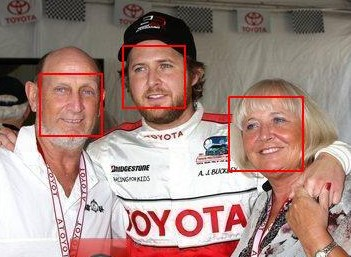
\includegraphics[width=0.55\textwidth]{images/image2a.jpg}
\end{center}
  \caption{Example of an image for which the face detector detects more than one face.}
\label{fig:validation}
\end{figure}

\end{tframe}


\begin{tframe}{Validation}

In order to resolve these errors and to evaluated the performance of the procedure, a method for visual validation was implemented.

\vspace{0.1in}

A \textbf{web application} was created for this purpose, thank to which are shown to a \textbf{user} the images associated to each identity and the results of the classification.

\vspace{0.1in}

The images with a \textbf{red overlay} represent the ones that the classifier consider not belonging to that identity.

\vspace{0.1in}

A \textbf{user} can interact with the web application, by browsing each identity and the images that are shown in a gallery; the user can also double click an image to \textbf{correct} the results of the classification. A user can also decide to completely remove an identity from the dataset.

\end{tframe}


\begin{tframe}{Validation}

\begin{figure}[h]
\begin{center}
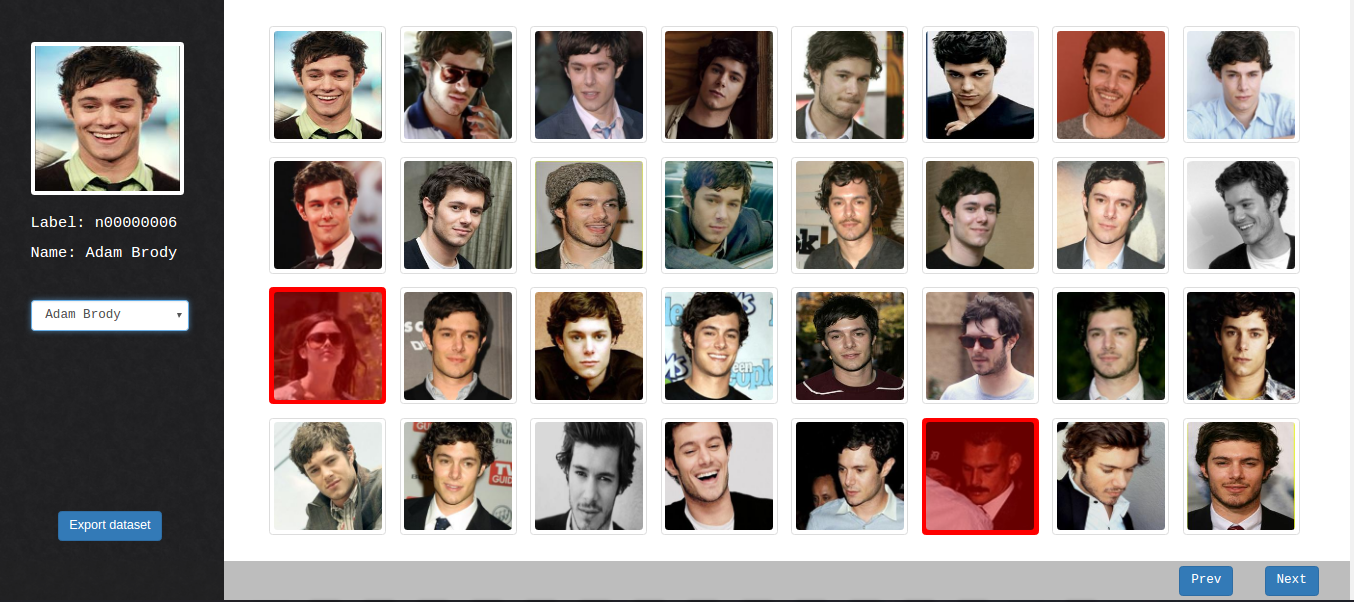
\includegraphics[width=1\textwidth]{images/image5.png}
\end{center}
  \caption{A screenshot of the implemented web application.}
\label{fig:validation}
\end{figure}

\end{tframe}